\subsection{Procesamiento}

Se tomaron en cuenta restricciones sobre el brazo robótico a controlar y los servomotores posicionales a los que se envían las instrucciones.

El tipo de brazo robótico a controlar tiene un diseño antropomórfico, lo que significa que se compone de articulaciones unidas entre sí; además es de dos grados de libertad, lo que implica que tiene exactamente dos articulaciones. Como lo que interesa es controlar la posición (y no la orientación), se restringió la cantidad de grados de libertad del brazo robótico a uno en cada unión; esto significa que en la unión de la base existe un grado de libertad, y el otro grado de libertad se encuentra en la unión entre la primera y la segunda articulación. Además, ambos grados de libertad se mueven de arriba hacia abajo. Para alcanzar todas las posiciones posibles en el espacio, existe un grado de libertad adicional en la base que rota el brazo robótico alrededor de su eje. La Figura \ref{fig:tipobrazo} muestra un ejemplo de un brazo robótico que cumple con estas restricciones.

\begin{figure}[htb]
	\centering
	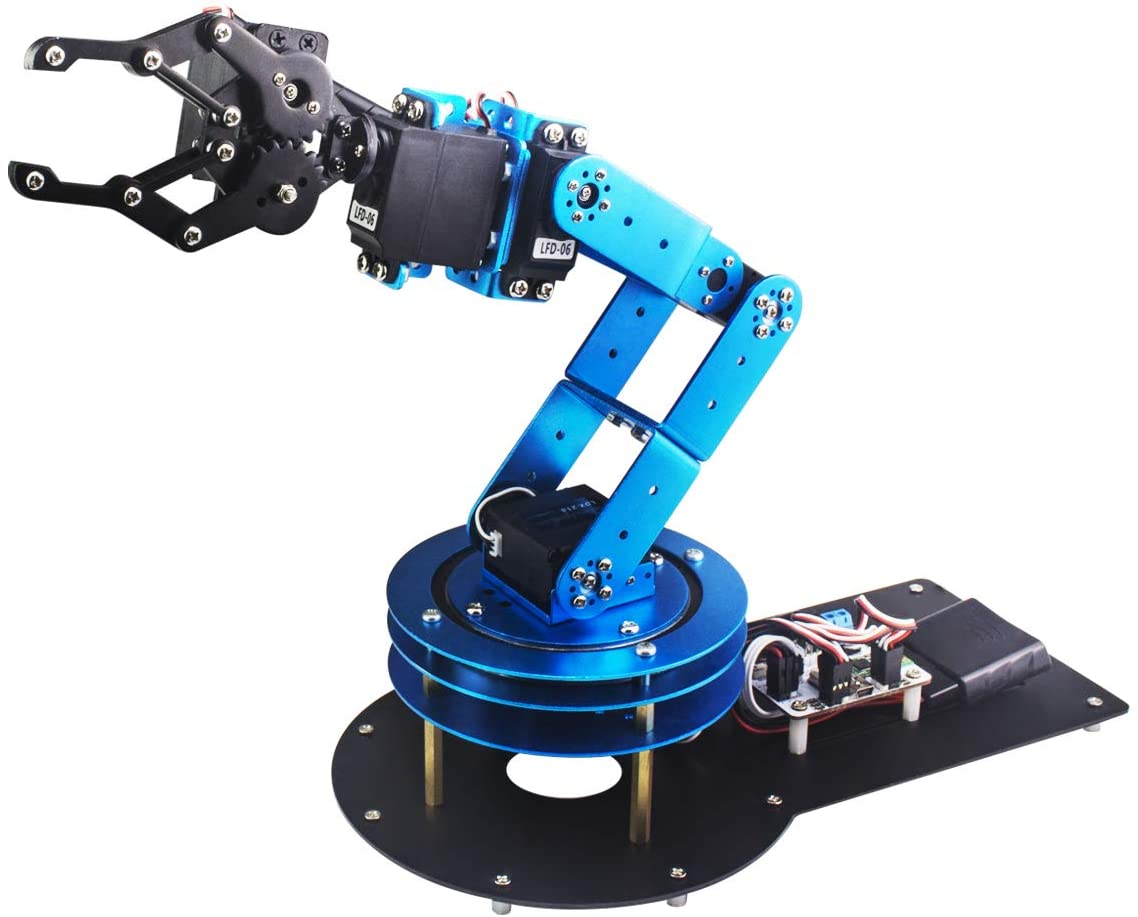
\includegraphics[scale=0.15]{tipobrazo.jpg}
	\caption{Brazo robótico de 2 DoF que cumple las restricciones impuestas}
	\label{fig:tipobrazo}
\end{figure}

El brazo robótico tiene la base en el suelo; esto significa que se puede mover dentro y en el contorno curvo de la mitad de una esfera con centro en la base del robot y de radio igual a la longitud del robot; debido a que la ortesis utilizada para localizar la posición tiene 42 cm de largo, ésta es la máxima longitud del brazo para el sistema. Los servomotores posicionales solo pueden moverse en ángulos discretos, en particular, enteros. Esto significa que pueden alcanzar 180 posiciones. Además, muchas posiciones finales son lo suficientemente cercanas entre sí como para considerar que se aproximan a la misma posición.  Para determinar la proximidad de las posiciones, se aplicó el siguiente criterio con distancia Euclidiana entre dos posiciones. Si $P_1 = (x_1, y_1, z_1)$ es un punto en el espacio tal que sus coordenadas son valores enteros y $P_2 = (x_2, y_2, z_2)$ es cualquier otro punto:

\begin{equation}
	d(P_1, P_2) = \sqrt{(x_2 - x_1)^2 + (y_2 - y_1)^2 + (z_2 - z_1)^2} <= \frac{\sqrt{2}}{2} \approx 0.707
\end{equation}

De este modo, se considera que aquellos puntos que tienen a lo más 0,707 cm de distancia euclidiana entre ellos llegan a la misma posición. Para el caso en el que una de las coordenadas del punto $P_2$ sea entera, su distancia euclidiana al punto $P_1$ más cercano será menor que o igual a 0,5 cm, de modo que el criterio se reducirá a ese valor máximo. Si las posiciones alcanzables son como el punto $P_1$ antes descrito, esto significa que las posiciones alcanzables dentro del volumen de la semiesfera donde se puede mover el brazo robótico se reducen, lo que optimiza la determinación de la posición final. Note que la imprecisión es a lo más de 0.707 cm. 

Podemos notar que muchas posiciones pueden ser alcanzadas por un brazo robótico de una determinada longitud de articulaciones con más de una combinación de ángulos; por ejemplo, si la base tiene 0°, y ambas articulaciones tienen 90° y 0°, respectivamente, se alcanza la misma posición que si la base tiene 180°, y ambas articulaciones tienen 90° y 180°, respectivamente. En particular, si colocamos un plano paralelo al diámetro de la semiesfera que la atraviese, podemos notar las configuraciones ``espejo'' que alcanzan la misma posición. De modo que se restringió el rango de movilidad de las articulaciones de 0 a 90° para reducir aún más el espacio de búsqueda; la base se mantuvo de 0 a 360°. 

Esto nos da las siguientes restricciones para generar el conjunto de datos:

\begin{itemize} 
	
	\item $\alpha_1, \alpha_2, \alpha_3 \in \mathbb{Z}$; El ángulo de la base es $ 0 \leq \alpha_1 \leq 360$, mientras que los ángulos de inclinación de las articulaciones son $ 0 \leq \alpha_2, \alpha_3 \leq 90$
	
	\item Las posiciones alcanzables $P = (x, y, z)$ son tales que $x,y,z \ in \mathbb{Z}$, y se asocian con un conjunto de combinaciones de longitudes $L_1, L_2$ y ángulos de inclinación $alpha_1, alpha_2$ que las alcanzan
	
\end{itemize}

Con base en lo anterior se generaron los datos, de modo que cada posición alcanzable se asociara con el conjunto de ángulos que generan la posición con menor distancia euclidiana al punto alcanzable.

Una vez obtenidos los grupos, se almacenaron en archivos binarios de acuerdo con la posicion especifica. De este modo, cuando se ingrese una posición $P(x,y,z)$ con longitudes $L_1, L_2$, primero, se determina el punto más cercano $P_i(x_i,y_i,z_i)$ a $P(x,y,z)$ tal que $x_i,y_i,z_i \in \mathbb{Z}$ de los 8 puntos que rodean a $P(x,y,z)$, si se considera esta posición dentro de un cubo (las esquinas $P_i(x_i,y_i,z_i)$ son parte de los puntos como $P_1$ revisados antes); posteriormente, se busca en el archivo binario donde se guardaron las posiciones con la misma coordenada $x_i$. Al iterar dentro del archivo,  si las longitudes asociadas a esos ángulos no difieren en más de 1 cm con las longitudes de entrada (también se invierten las longitudes), se sustituyen los ángulos $\alpha_1, \alpha_2, \alpha_3$, en las siguientes ecuaciones obtenidas de las matrices de rotación del brazo robótico que determinan la posición real si se toman esos ángulos de inclinación.:

\begin{equation}
	x = L_1 \cdot \cos(\alpha_2) \cdot \cos(\alpha_1) + L_2 \cdot \cos(\alpha_2 + \alpha_3) \cdot \cos(\alpha_1)
\end{equation}
	
\begin{equation}
	y = L_1 \cdot \cos(\alpha_2) \cdot \sin(\alpha_1) + L_2 \cdot \cos(\alpha_2 + \alpha_3) \cdot \sin(\alpha_1)
\end{equation}
	
\begin{equation}
	z = L_1 \cdot \sin(\alpha_2) + L_2 \cdot \sin(\alpha_2 + \alpha_3) \cdot \cos(\alpha_1)
\end{equation}

Y se determina la distancia euclidiana de la posición obtenida con la posición $P(x,y,z)$ de entrada. La combinación de ángulos $\alpha_1, \alpha_2, \alpha_3$ que tenga la menor distancia euclidiana, se toma como la salida de la etapa de Procesamiento.